\documentclass[12pt]{article}
\usepackage{fontspec}
\usepackage{fullpage}
\usepackage{hyperref}
\hypersetup{bookmarks=true,colorlinks=true,linkcolor=red,citecolor=blue,filecolor=magenta,urlcolor=cyan}
\usepackage{amsmath}
\usepackage{amssymb}
\usepackage{mathtools}
\usepackage{unicode-math}
\usepackage{tabularray}
\usepackage{tabularx}
\usepackage{booktabs}
\usepackage{caption}
\usepackage{graphics}
\usepackage{svg}
\usepackage{enumitem}
\usepackage{filecontents}
\usepackage[backend=bibtex]{biblatex}
\usepackage{url}
\setmathfont{Latin Modern Math}
\newcommand{\gt}{\ensuremath >}
\newcommand{\lt}{\ensuremath <}
\newlist{symbDescription}{description}{1}
\setlist[symbDescription]{noitemsep, topsep=0pt, parsep=0pt, partopsep=0pt}
\bibliography{bibfile}
\title{Software Requirements Specification for Chemistry Code}
\author{Samuel J. Crawford}
\begin{document}
\maketitle
\tableofcontents
\newpage
\section{Reference Material}
\label{Sec:RefMat}
This section records information for easy reference.

\subsection{Table of Symbols}
\label{Sec:ToS}
The symbols used in this document are summarized in the \hyperref[Table:ToS]{Table of Symbols} along with their units. The symbols are listed in alphabetical order.

\begin{longtblr}
[caption={Table of Symbols}]
{colspec={l l l}, rowhead=1, hline{1,Z}=\heavyrulewidth, hline{2}=\lightrulewidth}
\textbf{Symbol} & \textbf{Description} & \textbf{Units}
\\
$\symbf{0}$ & Zero vector & --
\\
$\symbf{1}$ & Unary vector & --
\\
$\symbf{A}$ & Generic matrix & --
\\
$\symbf{b}$ & Generic vector & --
\\
$C$ & Compound data type & --
\\
$c$ & Generic compound & --
\\
${c^{r}}$ & Generic record of a compound & --
\\
$\symbf{c}$ & Generic vector & --
\\
$\text{count}$ & Count of an element in a compound & --
\\
$E$ & Element data type & --
\\
$e$ & Generic element & --
\\
$\text{elems}$ & Set of elements in a chemical reaction & --
\\
$i$ & Generic integer & --
\\
$j$ & Generic integer & --
\\
$\text{MAINTAIN_FRAC}$ & Maintainability fraction & --
\\
$\symbf{Q}$ & Matrix representation of a chemical equation & --
\\
${q_{\text{ij}}}$ & Element of $\symbf{Q}$ & --
\\
$R$ & Reaction data type & --
\\
$r$ & Generic reaction & --
\\
${r_{\text{in}}}$ & Representation of a chemical equation & --
\\
$x$ & Generic real number & --
\\
$\symbf{x}$ & Generic vector & --
\\
$y$ & Generic integer & --
\label{Table:ToS}
\end{longtblr}
\subsection{Abbreviations and Acronyms}
\label{Sec:TAbbAcc}
\begin{longtblr}
[caption={Abbreviations and Acronyms}]
{colspec={l l}, rowhead=1, hline{1,Z}=\heavyrulewidth, hline{2}=\lightrulewidth}
\textbf{Abbreviation} & \textbf{Full Form}
\\
A & Assumption
\\
ChemCode & Chemistry Code
\\
DD & Data Definition
\\
IM & Instance Model
\\
IUPAC & International Union of Pure and Applied Chemistry
\\
ODE & Ordinary Differential Equation
\\
R & Requirement
\\
SRS & Software Requirements Specification
\\
TM & Theoretical Model
\\
UC & Unlikely Change
\label{Table:TAbbAcc}
\end{longtblr}
\section{Introduction}
\label{Sec:Intro}
Chemical equations are common ways of representing chemical reactions (\hyperref[Figure:physSysFig]{Fig:physSysFig} shows an example of a chemical equation). Subscripts indicate the number of atoms of each element present in the given chemical compound. A chemical equation is ``balanced'' if there are the same number of atoms of each element before and after the reaction takes place, which satisfies the Law of Conservation of Mass. Chemical equations are balanced by introducing coefficients before each chemical formula (this coefficient may be ``1'', in which case is implicit and not added to the equation). We want a tool to balance chemical equations automatically to improve the productivity of scientists and engineers and reduce the potential for human error. This program should balance a given chemical equation if it is feasible and if it is not, it should provide a message communicating this to the user. The program that performs these tasks as documented here will be called Chemistry Code (ChemCode).

The following section provides an overview of the Software Requirements Specification (SRS) for ChemCode. This section explains the purpose of this document, the scope of the requirements, the characteristics of the intended reader, and the organization of the document.

\subsection{Purpose of Document}
\label{Sec:DocPurpose}
The primary purpose of this document is to record the requirements of ChemCode. Goals, assumptions, theoretical models, definitions, and other model derivation information are specified, allowing the reader to fully understand and verify the purpose and scientific basis of ChemCode. With the exception of \hyperref[Sec:SysConstraints]{system constraints}, this SRS will remain abstract, describing what problem is being solved, but not how to solve it.

This document will be used as a starting point for subsequent development phases, including writing the design specification and the software verification and validation plan. The design document will show how the requirements are to be realized, including decisions on the numerical algorithms and programming environment. The verification and validation plan will show the steps that will be used to increase confidence in the software documentation and the implementation. Although the SRS fits in a series of documents that follow the so-called waterfall model, the actual development process is not constrained in any way. Even when the waterfall model is not followed, as Parnas and Clements point out \cite{parnasClements1986}, the most logical way to present the documentation is still to ``fake'' a rational design process.

\subsection{Scope of Requirements}
\label{Sec:ReqsScope}
The scope of the requirements includes all inputted chemical equations where the total number of chemical compounds is at most one more than the total number of elements. These chemical equations will be balanced with integer coefficients. The scope also includes all inputted chemical formulas that describe real chemical compounds, are formatted following a set of conventions, and only consist of atomic symbols and subscripts (including the fractional subscripts in nonstoichiometric compounds).

\subsection{Characteristics of Intended Reader}
\label{Sec:ReaderChars}
Reviewers of this documentation should have an understanding of high school chemistry (namely stochiometry) and third year linear optimization (namely integer programming). The users of ChemCode can have a lower level of expertise, as explained in \hyperref[Sec:UserChars]{Sec:User Characteristics}.

\subsection{Organization of Document}
\label{Sec:DocOrg}
The organization of this document follows the template for an SRS for scientific computing software proposed by \cite{koothoor2013}, \cite{smithLai2005}, \cite{smithEtAl2007}, and \cite{smithKoothoor2016}. The presentation follows the standard pattern of presenting goals, theories, definitions, and assumptions. For readers that would like a more bottom up approach, they can start reading the \hyperref[Sec:IMs]{instance models} and trace back to find any additional information they require.

The \hyperref[Sec:GoalStmt]{goal statements} are refined to the theoretical models and the \hyperref[Sec:TMs]{theoretical models} to the \hyperref[Sec:IMs]{instance models}.

\section{General System Description}
\label{Sec:GenSysDesc}
This section provides general information about the system. It identifies the interfaces between the system and its environment, describes the user characteristics, and lists the system constraints.

\subsection{System Context}
\label{Sec:SysContext}
\hyperref[Figure:sysCtxFig]{Fig:sysCtxFig} shows the system context. A circle represents an external entity outside the software, the user in this case. A rectangle represents the software system itself (ChemCode). Arrows are used to show the data flow between the system and its environment.

\begin{figure}
\begin{center}
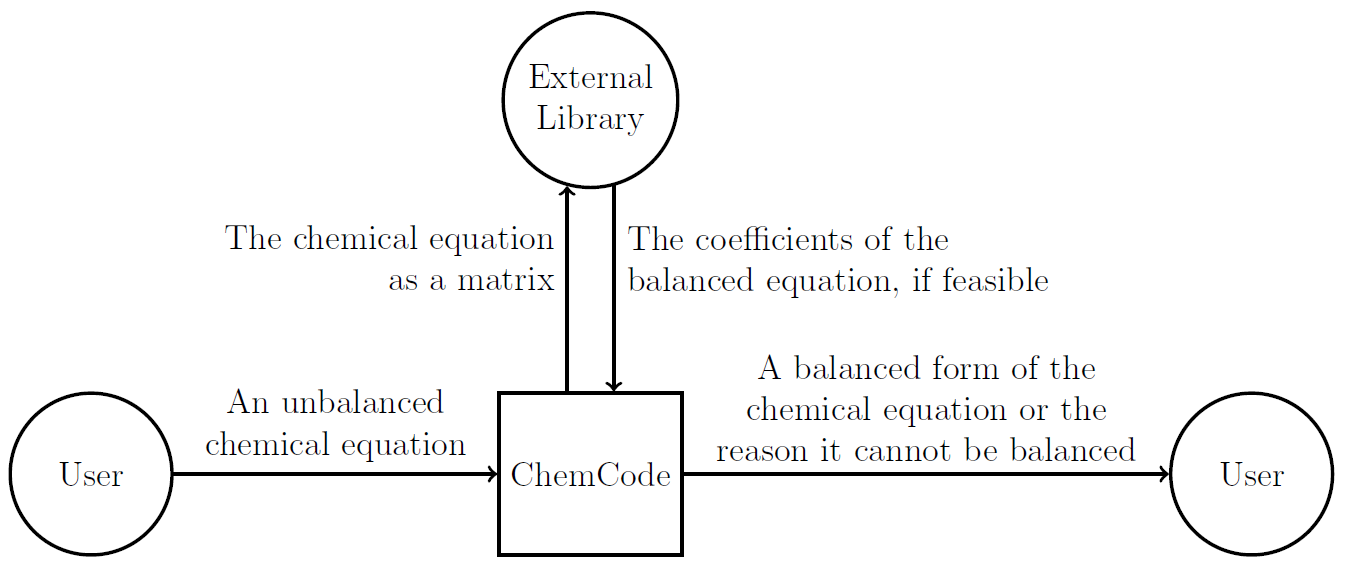
\includegraphics[width=\textwidth]{../../../../datafiles/chemcode/sysCtxFig.png}
\caption{System Context}
\label{Figure:sysCtxFig}
\end{center}
\end{figure}
The interaction between the product and the user is through a user interface. The responsibilities of the user and the system are as follows:

\begin{itemize}
\item{User Responsibilities}
\begin{itemize}
\item{Provide an unbalanced chemical equation, ensuring conformation to input data format required by ChemCode}
\item{Ensure required \hyperref[Sec:Assumps]{software assumptions} are appropriate for the problem to which the user is applying the software}
\end{itemize}
\item{ChemCode Responsibilities}
\begin{itemize}
\item{Detect data type mismatch, such as a string of characters instead of a floating point number}
\item{Format the inputted chemical equation as a matrix}
\item{If the inputted chemical equation is feasible, find its balanced form with the smallest possible whole number coefficients}
\end{itemize}
\item{External Library Responsibilities}
\begin{itemize}
\item{Solve the integer linear programming problem for the inputted chemical equation}
\end{itemize}
\end{itemize}
\subsection{User Characteristics}
\label{Sec:UserChars}
The end user of ChemCode should have an understanding of high school chemistry (namely stochiometry).

\subsection{System Constraints}
\label{Sec:SysConstraints}
ChemCode will be developed using Drasil \cite{drasilSource}, ``a framework for generating high-quality documentation and code for Scientific Computing Software'' \cite{maclachlan2021}, with the goal of extending it by adding concepts relevant to the problem outlined in the \hyperref[Sec:ProbDesc]{problem description}. Since Drasil is built on the idea of reusability, external libraries will be used to solve the integer programming problems. This was previously done with ordinary differential equation (ODE) solvers, since ``creating a complete ODE solver in Drasil would take considerable time, and there are already many reliable external libraries ... tested by long use'' \cite[(pg. 24)]{chen2022}. These rationales also apply to ILP solvers.

\section{Specific System Description}
\label{Sec:SpecSystDesc}
This section first presents the problem description, which gives a high-level view of the problem to be solved. This is followed by the solution characteristics specification, which presents the assumptions, theories, and definitions that are used.

\subsection{Problem Description}
\label{Sec:ProbDesc}
A system is needed to balance chemical equations so they can be useful for other computations \cite{lund2023}. Additionally, since molecules only exist in positive integer quantities (since dividing a molecule changes it into different molecules), the coefficients used to balance the chemical equation should be whole numbers, and by convention should be as small as possible \cite{lund2023}. There are some cases where the coefficients are not integers (see \cite{nonIntCoeffSource}), but this is not in the scope of this program.

\subsubsection{Terminology and Definitions}
\label{Sec:TermDefs}
This subsection provides a list of terms that are used in the subsequent sections and their meaning, with the purpose of reducing ambiguity and making it easier to correctly understand the requirements.

\begin{itemize}
\item{Balanced: (Referring to a chemical equation) following the Law of Conservation of Matter (\hyperref[TM:lawConsMass]{TM:lawConsMass}).}
\item{Compound: A molecule made up of more than one atom, which may or may not be of different elements.}
\item{Element: The group of all atoms with the same number of protons in the atomic nucleus. For example, all atoms with one proton are hydrogen atoms.}
\item{Equation: A textual representation of a chemical reaction.}
\item{Feasible: (Referring to a chemical equation) able to be balanced.}
\item{Formula: A textual representation of a chemical compound.}
\item{Hydrate: ``a compound formed by the chemical combination of water and some other substance in a definite molecular ratio'' \cite{hydrateSource}.}
\item{Isotope: An atom that is the same element as another but has a different number of neutrons \cite{lund2023}.}
\item{Nonstoichiometric compound: ``Any solid chemical compound in which the numbers of atoms of the elements present cannot be expressed as a ratio of small positive integers''.}
\item{Polyatomic ion: A group of atoms ``bonded together that carr[ies] an overall electric charge'' \cite{lund2023}.}
\item{Polymer: A macromolecule ``formed by the chemical bonding of large numbers of smaller molecules'' \cite{polymerSource}.}
\item{Product: A substance formed by a chemical reaction.}
\item{Reactant: A substance involved in and changed by a chemical reaction.}
\item{Reaction: An interaction between different types of matter that results in at least one new substance being formed \cite{lund2023}.}
\item{Stoichiometry: ``The calculation of the quantities of reactants or products in a chemical reaction using the relationships found in a balanced chemical equation'' \cite[(pg. 337)]{lund2023}.}
\end{itemize}
\subsubsection{Physical System Description}
\label{Sec:PhysSyst}
The physical system of ChemCode, as shown in \hyperref[Figure:physSysFig]{Fig:physSysFig}, includes the following elements:

\begin{itemize}
\item[PS1:]{The reactants of a given chemical reaction.}
\item[PS2:]{The products of the same chemical reaction.}
\end{itemize}
\begin{figure}
\begin{center}
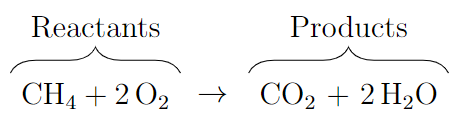
\includegraphics[width=\textwidth]{../../../../datafiles/chemcode/physSysFig.png}
\caption{Physical System Description}
\label{Figure:physSysFig}
\end{center}
\end{figure}
\hyperref[Figure:physSysFig]{Fig:physSysFig} was partially generated by ChatGPT.

\subsubsection{Goal Statements}
\label{Sec:GoalStmt}
Given a representation of a chemical equation, the goal statement is:

\begin{itemize}
\item[findBalancedForm:\phantomsection\label{findBalancedForm}]{Find its balanced form with the smallest positive integer coefficients if it is feasible.}
\end{itemize}
\subsection{Solution Characteristics Specification}
\label{Sec:SolCharSpec}
The instance models that govern ChemCode are presented in the \hyperref[Sec:IMs]{Instance Model Section}. The information to understand the meaning of the instance models and their derivation is also presented, so that the instance models can be verified.

\subsubsection{Assumptions}
\label{Sec:Assumps}
This section simplifies the original problem and helps in developing the theoretical models by filling in the missing information for the physical system. The assumptions refine the scope by providing more detail.

\begin{itemize}
\item[elemCompDiff:\phantomsection\label{elemCompDiff}]{For all chemical equations, the total number of chemical compounds is at most one more than the total number of elements. (RefBy: \hyperref[allEqsPermitted]{UC:allEqsPermitted}.)}
\item[validForms:\phantomsection\label{validForms}]{All inputted chemical formulas describe real chemical compounds. (RefBy: \hyperref[checkValidForms]{UC:checkValidForms}.)}
\item[validEqns:\phantomsection\label{validEqns}]{All inputted chemical equations describe real chemical reactions. (RefBy: \hyperref[checkValidEqns]{UC:checkValidEqns}.)}
\item[correctInputFormat:\phantomsection\label{correctInputFormat}]{All inputted chemical formulas follow the conventions laid out in \cite{inorganicIUPAC} and \cite{organicIUPAC} by the International Union of Pure and Applied Chemistry (IUPAC). (RefBy: \hyperref[incInputFormat]{LC:incInputFormat}.)}
\item[simpleForms:\phantomsection\label{simpleForms}]{All inputted chemical formulas only consist of atomic symbols and subscripts. This means that they cannot contain dots, parentheses, hyphens, or superscripts, so hydrates, polymers, and formulas with isotopes and some with polyatomic ions will not be present in inputted chemical equations. (RefBy: \hyperref[complexForms]{LC:complexForms}.)}
\item[intCoeffs:\phantomsection\label{intCoeffs}]{All chemical equations will be balanced using integer coefficients. (RefBy: \hyperref[nonintCoeffs]{UC:nonintCoeffs}.)}
\end{itemize}
\subsubsection{Theoretical Models}
\label{Sec:TMs}
This section focuses on the general equations and laws that ChemCode is based on.

\medskip
\noindent
\begin{minipage}{\textwidth}
\begin{tabular}{>{\raggedright}p{0.13\textwidth}>{\raggedright\arraybackslash}p{0.82\textwidth}}
\toprule \textbf{Refname} & \textbf{TM:canonIntLinProg}
\phantomsection 
\label{TM:canonIntLinProg}
\\ \midrule
Label & Canonical integer linear program
        
\\ \midrule
Equation & \begin{displaymath}
           \symbf{c} \symbf{x}
           \end{displaymath}
           \begin{displaymath}
           \symbf{A} \symbf{x}\leq{}\symbf{b}
           \end{displaymath}
           \begin{displaymath}
           \symbf{x}\geq{}\symbf{0}
           \end{displaymath}
           \begin{displaymath}
           \symbf{x}\in{}\mathbb{Z}^{n}
           \end{displaymath}
\\ \midrule
Description & \begin{symbDescription}
              \item{$\symbf{c}$ is the generic vector (Unitless)}
              \item{$\symbf{x}$ is the generic vector (Unitless)}
              \end{symbDescription}
              \begin{symbDescription}
              \item{$\symbf{A}$ is the generic matrix (Unitless)}
              \item{$\symbf{x}$ is the generic vector (Unitless)}
              \item{$\symbf{b}$ is the generic vector (Unitless)}
              \end{symbDescription}
              \begin{symbDescription}
              \item{$\symbf{x}$ is the generic vector (Unitless)}
              \item{$\symbf{0}$ is the zero vector (Unitless)}
              \end{symbDescription}
              \begin{symbDescription}
              \item{$\symbf{x}$ is the generic vector (Unitless)}
              \end{symbDescription}
\\ \midrule
Notes & The above equation gives the canonical form of an integer linear program, which is ``a mathematical optimization or feasibility program in which some or all of the variables are restricted to be integers [and] the objective function and the constraints (other than the integer constraints) are linear'' \cite{ilpWiki}.
        
        The values of $\symbf{x}$ are unknown and will be solved for.
        
\\ \midrule
Source & \cite{ilpWiki}
         
\\ \midrule
RefBy & \hyperref[IM:chemEqIntLinProg]{IM:chemEqIntLinProg}
        
\\ \bottomrule
\end{tabular}
\end{minipage}

\medskip
\noindent
\begin{minipage}{\textwidth}
\begin{tabular}{>{\raggedright}p{0.13\textwidth}>{\raggedright\arraybackslash}p{0.82\textwidth}}
\toprule \textbf{Refname} & \textbf{TM:lawConsMass}
\phantomsection 
\label{TM:lawConsMass}
\\ \midrule
Label & Law of conservation of mass
        
\\ \midrule
Equation & \begin{displaymath}
           \forall{}\,e\in{}E,r\in{}R\text{ | }\displaystyle\sum{\text{count}\left(e,r_{i}\text{.comp}\right) {r\text{.reac}}_{i}\text{.coeff}}=\displaystyle\sum{\text{count}\left(e,r_{i}\text{.comp}\right) {r\text{.prod}}_{i}\text{.coeff}}
           \end{displaymath}
\\ \midrule
Description & \begin{symbDescription}
              \item{$\text{count}$ is the count of an element in a compound (Unitless)}
              \item{$e$ is the generic element (Unitless)}
              \item{$r$ is the generic reaction (Unitless)}
              \item{$i$ is the generic integer (Unitless)}
              \end{symbDescription}
\\ \midrule
Notes & This law states that ``matter can neither be created nor destroyed in a chemical reaction ... but it may change forms to other substances'' \cite[(pg. 112)]{lund2023}.
        
        The above equation assumes that $r$ is balanced.
        
\\ \midrule
Source & \cite{lund2023}
         
\\ \midrule
RefBy & 
\\ \bottomrule
\end{tabular}
\end{minipage}

\subsubsection{General Definitions}
\label{Sec:GDs}
There are no general definitions.

\subsubsection{Data Definitions}
\label{Sec:DDs}
This section collects and defines all the data needed to build the instance models.

\medskip
\noindent
\begin{minipage}{\textwidth}
\begin{tabular}{>{\raggedright}p{0.13\textwidth}>{\raggedright\arraybackslash}p{0.82\textwidth}}
\toprule \textbf{Refname} & \textbf{DD:elementType}
\phantomsection 
\label{DD:elementType}
\\ \midrule
Label & Element data type
        
\\ \midrule
Symbol & $E$
         
\\ \midrule
Equation & \begin{displaymath}
           E=\{\text{H},\text{He},\text{Li},\text{Be},\text{B},\text{C},\text{N},\text{O},\text{F},\text{Ne},\text{Na},\text{Mg},\text{Al},\text{Si},\text{P},\text{S},\text{Cl},\text{Ar},\text{K},\text{Ca},\text{Sc},\text{Ti},\text{V},\text{Cr},\text{Mn},\text{Fe},\text{Co},\text{Ni},\text{Cu},\text{Zn},\text{Ga},\text{Ge},\text{As},\text{Se},\text{Br},\text{Kr},\text{Rb},\text{Sr},\text{Y},\text{Zr},\text{Nb},\text{Mo},\text{Tc},\text{Ru},\text{Rh},\text{Pd},\text{Ag},\text{Cd},\text{In},\text{Sn},\text{Sb},\text{Te},\text{I},\text{Xe},\text{Cs},\text{Ba},\text{La},\text{Ce},\text{Pr},\text{Nd},\text{Pm},\text{Sm},\text{Eu},\text{Gd},\text{Tb},\text{Dy},\text{Ho},\text{Er},\text{Tm},\text{Yb},\text{Lu},\text{Hf},\text{Ta},\text{W},\text{Re},\text{Os},\text{Ir},\text{Pt},\text{Au},\text{Hg},\text{Tl},\text{Pb},\text{Bi},\text{Po},\text{At},\text{Rn},\text{Fr},\text{Ra},\text{Ac},\text{Th},\text{Pa},\text{U},\text{Np},\text{Pu},\text{Am},\text{Cm},\text{Bk},\text{Cf},\text{Es},\text{Fm},\text{Md},\text{No},\text{Lr},\text{Rf},\text{Db},\text{Sg},\text{Bh},\text{Hs},\text{Mt},\text{Ds},\text{Rg},\text{Cn},\text{Nh},\text{Fl},\text{Mc},\text{Lv},\text{Ts},\text{Og}\}
           \end{displaymath}
\\ \midrule
Description & \begin{symbDescription}
              \item{$E$ is the element data type (Unitless)}
              \end{symbDescription}
\\ \midrule
Notes & A type representing each element from \cite{elemListWiki}.
        
\\ \midrule
Source & \cite{smithChemSpec}
         
\\ \midrule
RefBy & 
\\ \bottomrule
\end{tabular}
\end{minipage}

\medskip
\noindent
\begin{minipage}{\textwidth}
\begin{tabular}{>{\raggedright}p{0.13\textwidth}>{\raggedright\arraybackslash}p{0.82\textwidth}}
\toprule \textbf{Refname} & \textbf{DD:compoundType}
\phantomsection 
\label{DD:compoundType}
\\ \midrule
Label & Compound data type
        
\\ \midrule
Symbol & $C$
         
\\ \midrule
Equation & \begin{displaymath}
           C=\text{sequence of}\,\text{record of}\,\left(\text{elem}\in{}E,\,\text{count}\in{}\mathbb{R}\right)
           \end{displaymath}
\\ \midrule
Description & \begin{symbDescription}
              \item{$C$ is the compound data type (Unitless)}
              \end{symbDescription}
\\ \midrule
Notes & A type representing a compound.
        
\\ \midrule
Source & --
         
\\ \midrule
RefBy & 
\\ \bottomrule
\end{tabular}
\end{minipage}

\medskip
\noindent
\begin{minipage}{\textwidth}
\begin{tabular}{>{\raggedright}p{0.13\textwidth}>{\raggedright\arraybackslash}p{0.82\textwidth}}
\toprule \textbf{Refname} & \textbf{DD:reactionType}
\phantomsection 
\label{DD:reactionType}
\\ \midrule
Label & Reaction data type
        
\\ \midrule
Symbol & $R$
         
\\ \midrule
Equation & \begin{displaymath}
           R=\text{record of}\,\left(\text{prod}\in{}\text{sequence of}\,\text{record of}\,\left(\text{comp}\in{}C,\,\text{coeff}\in{}\mathbb{Z}\right),\,\text{reac}\in{}\text{sequence of}\,\text{record of}\,\left(\text{comp}\in{}C,\,\text{coeff}\in{}\mathbb{Z}\right)\right)
           \end{displaymath}
\\ \midrule
Description & \begin{symbDescription}
              \item{$R$ is the reaction data type (Unitless)}
              \end{symbDescription}
\\ \midrule
Notes & A type representing a reaction.
        
\\ \midrule
Source & --
         
\\ \midrule
RefBy & 
\\ \bottomrule
\end{tabular}
\end{minipage}

\medskip
\noindent
\begin{minipage}{\textwidth}
\begin{tabular}{>{\raggedright}p{0.13\textwidth}>{\raggedright\arraybackslash}p{0.82\textwidth}}
\toprule \textbf{Refname} & \textbf{DD:countFunc}
\phantomsection 
\label{DD:countFunc}
\\ \midrule
Label & Count of an element in a compound
        
\\ \midrule
Symbol & $\text{count}$
         
\\ \midrule
Equation & \begin{displaymath}
           \text{count}\left(e,c\right)=\begin{cases}
                                        {c^{r}}\text{.count}\,\text{such that }\,{c^{r}}\in{}c\land{}{c^{r}}\text{.elem}=e, & \exists{}\,{{c^{r}}\in{}\text{record of}\,\left(\text{elem}\in{}E,\,\text{count}\in{}\mathbb{R}\right)}\text{ | }{c^{r}}\in{}c\land{}{c^{r}}\text{.elem}=e\\
                                        0, & \neg{}\exists{}\,{{c^{r}}\in{}\text{record of}\,\left(\text{elem}\in{}E,\,\text{count}\in{}\mathbb{R}\right)}\text{ | }{c^{r}}\in{}c\land{}{c^{r}}\text{.elem}=e
                                        \end{cases}
           \end{displaymath}
\\ \midrule
Description & \begin{symbDescription}
              \item{$\text{count}$ is the count of an element in a compound (Unitless)}
              \item{${c^{r}}$ is the generic record of a compound (Unitless)}
              \item{$c$ is the generic compound (Unitless)}
              \item{$e$ is the generic element (Unitless)}
              \end{symbDescription}
\\ \midrule
Notes & The output represents the number of atoms of a given element $e$ (of type $E$) in a given compound $c$ (of type $C$).
        
\\ \midrule
Source & --
         
\\ \midrule
RefBy & 
\\ \bottomrule
\end{tabular}
\end{minipage}

\medskip
\noindent
\begin{minipage}{\textwidth}
\begin{tabular}{>{\raggedright}p{0.13\textwidth}>{\raggedright\arraybackslash}p{0.82\textwidth}}
\toprule \textbf{Refname} & \textbf{DD:elemsFunc}
\phantomsection 
\label{DD:elemsFunc}
\\ \midrule
Label & Set of elements in a chemical reaction
        
\\ \midrule
Symbol & $\text{elems}$
         
\\ \midrule
Equation & \begin{displaymath}
           \text{elems}\left(r\right)=\{e\in{}E\text{ | }\exists{}\,c\in{}C,y\in{}\mathbb{Z},x\in{}\mathbb{R}\text{ | }\left(\left(c,y\right)\in{}r\text{.prod}\lor{}\left(c,y\right)\in{}r\text{.reac}\right)\land{}\left(e,x\right)\in{}c\}
           \end{displaymath}
\\ \midrule
Description & \begin{symbDescription}
              \item{$\text{elems}$ is the set of elements in a chemical reaction (Unitless)}
              \item{$e$ is the generic element (Unitless)}
              \item{$c$ is the generic compound (Unitless)}
              \item{$y$ is the generic integer (Unitless)}
              \item{$x$ is the generic real number (Unitless)}
              \item{$r$ is the generic reaction (Unitless)}
              \end{symbDescription}
\\ \midrule
Notes & The output represents the set of elements that occur in a given chemical equation $r$ (of type $R$).
        
\\ \midrule
Source & --
         
\\ \midrule
RefBy & 
\\ \bottomrule
\end{tabular}
\end{minipage}

\subsubsection{Instance Models}
\label{Sec:IMs}
This section transforms the problem defined in the \hyperref[Sec:ProbDesc]{problem description} into one which is expressed in mathematical terms. It uses concrete symbols defined in the \hyperref[Sec:DDs]{data definitions} to replace the abstract symbols in the models identified in \hyperref[Sec:TMs]{theoretical models} and \hyperref[Sec:GDs]{general definitions}.

\medskip
\noindent
\begin{minipage}{\textwidth}
\begin{tabular}{>{\raggedright}p{0.13\textwidth}>{\raggedright\arraybackslash}p{0.82\textwidth}}
\toprule \textbf{Refname} & \textbf{IM:matRepresentation}
\phantomsection 
\label{IM:matRepresentation}
\\ \midrule
Label & Matrix representation of a chemical equation
        
\\ \midrule
Input & ${r_{\text{in}}}$
        
\\ \midrule
Output & $\symbf{Q}$
         
\\ \midrule
Equation & \begin{displaymath}
           \symbf{Q}=\text{the matrix such that}\,\forall{}\,i\in{}\mathbb{Z},j\in{}\mathbb{Z}\text{ | }0\leq{}i\lt{}|\text{elems}\left({r_{\text{in}}}\right)|\land{}0\leq{}j\lt{}|{r_{\text{in}}}\text{.reac}|+|{r_{\text{in}}}\text{.prod}|\implies{}{q_{\text{ij}}}=\begin{cases}
                                                                                                                                                                                                                                                                        \text{count}\left({\text{elems}\left({r_{\text{in}}}\right)}_{i},{{r_{\text{in}}}\text{.reac}}_{j}\text{.comp}\right), & j\lt{}|{r_{\text{in}}}\text{.reac}|\\
                                                                                                                                                                                                                                                                        -\left(\text{count}\left({\text{elems}\left({r_{\text{in}}}\right)}_{i},{{r_{\text{in}}}\text{.prod}}_{j-|{r_{\text{in}}}\text{.reac}|}\text{.comp}\right)\right), & \neg{}j\lt{}|{r_{\text{in}}}\text{.reac}|
                                                                                                                                                                                                                                                                        \end{cases}
           \end{displaymath}
\\ \midrule
Description & \begin{symbDescription}
              \item{$\symbf{Q}$ is the matrix representation of a chemical equation (Unitless)}
              \item{$i$ is the generic integer (Unitless)}
              \item{$\text{elems}$ is the set of elements in a chemical reaction (Unitless)}
              \item{${r_{\text{in}}}$ is the representation of a chemical equation (Unitless)}
              \item{$j$ is the generic integer (Unitless)}
              \item{${q_{\text{ij}}}$ is the element of $\symbf{Q}$ (Unitless)}
              \item{$\text{count}$ is the count of an element in a compound (Unitless)}
              \end{symbDescription}
\\ \midrule
Source & --
         
\\ \midrule
RefBy & 
\\ \bottomrule
\end{tabular}
\end{minipage}

\medskip
\noindent
\begin{minipage}{\textwidth}
\begin{tabular}{>{\raggedright}p{0.13\textwidth}>{\raggedright\arraybackslash}p{0.82\textwidth}}
\toprule \textbf{Refname} & \textbf{IM:chemEqIntLinProg}
\phantomsection 
\label{IM:chemEqIntLinProg}
\\ \midrule
Label & Integer linear program for a chemical equation
        
\\ \midrule
Input & $\symbf{Q}$
        
\\ \midrule
Output & $\symbf{x}$
         
\\ \midrule
Equation & \begin{displaymath}
           \begin{aligned}
            & \text{minimize} &  & \symbf{1}\cdot{}\symbf{x}\\
            & \text{subject to} &  & \symbf{Q} \symbf{x}=\symbf{0},\\
            & \, &  & \symbf{x}\gt{}\symbf{0},\\
            & \text{and} &  & \symbf{x}\in{}\mathbb{Z}^{n}
           \end{aligned}
           \end{displaymath}
\\ \midrule
Description & \begin{symbDescription}
              \item{$\symbf{1}$ is the unary vector (Unitless)}
              \item{$\symbf{x}$ is the generic vector (Unitless)}
              \item{$\symbf{Q}$ is the matrix representation of a chemical equation (Unitless)}
              \item{$\symbf{0}$ is the zero vector (Unitless)}
              \end{symbDescription}
\\ \midrule
Notes & This is a specific instance of the ILP from \hyperref[TM:canonIntLinProg]{TM:canonIntLinProg} with $\symbf{A}=\symbf{Q}$, $\symbf{b}=\symbf{0}$, and $\symbf{c}=\symbf{1}$. The goal and constraints are also modified.
        
\\ \midrule
Source & --
         
\\ \midrule
RefBy & \hyperref[accurate]{NFR:Accurate}
        
\\ \bottomrule
\end{tabular}
\end{minipage}

\section{Requirements}
\label{Sec:Requirements}
This section provides the functional requirements, the tasks and behaviours that the software is expected to complete, and the non-functional requirements, the qualities that the software is expected to exhibit.

\subsection{Functional Requirements}
\label{Sec:FRs}
This section provides the functional requirements, the tasks and behaviours that the software is expected to complete.

\begin{itemize}
\item[Input-Values:\phantomsection\label{inputValues}]{Input the values from \hyperref[Table:ReqInputs]{Tab:ReqInputs}.}
\item[Convert-to-Matrix:\phantomsection\label{convertMatrix}]{Convert the inputted chemical equation to matrix form.}
\item[Feasible-Output:\phantomsection\label{feasOut}]{If the inputted chemical equation is feasible, output its balanced form with the smallest positive integer coefficients possible.}
\item[Infeasible-Output:\phantomsection\label{infeasOut}]{If the inputted chemical equation is infeasible, output a descriptive message.}
\end{itemize}
\begin{longtblr}
[caption={Required Inputs following \hyperref[inputValues]{FR:Input-Values}}]
{colspec={l l l}, rowhead=1, hline{1,Z}=\heavyrulewidth, hline{2}=\lightrulewidth}
\textbf{Symbol} & \textbf{Description} & \textbf{Units}
\\
${r_{\text{in}}}$ & Representation of a chemical equation & --
\label{Table:ReqInputs}
\end{longtblr}
\subsection{Non-Functional Requirements}
\label{Sec:NFRs}
This section provides the non-functional requirements, the qualities that the software is expected to exhibit.

\begin{itemize}
\item[Accurate:\phantomsection\label{accurate}]{Chemical equations are only useful if they are balanced \cite{lund2023}, so computed coefficients from \hyperref[IM:chemEqIntLinProg]{IM:chemEqIntLinProg} should be exact.}
\item[Verifiable:\phantomsection\label{verifiable}]{The code is tested following the Verification and Validation (VnV) Plan.}
\item[Understandable:\phantomsection\label{understandable}]{A new intended user (as described by \hyperref[Sec:UserChars]{Sec:User Characteristics}) is able to learn how to use ChemCode in an acceptable amount of time, as measured by the procedure in Section 10 of the VnV Plan.}
\item[Usable:\phantomsection\label{usable}]{An intended user (as described by \hyperref[Sec:UserChars]{Sec:User Characteristics}) finds ChemCode easy to use, as measured by the procedure in Section 11 of the VnV Plan.}
\item[Reusable:\phantomsection\label{reusable}]{The code is modularized.}
\item[Maintainable:\phantomsection\label{maintainable}]{The development time for any of the likely changes will not exceed $\text{MAINTAIN_FRAC}$ of the original development time.}
\item[Portable:\phantomsection\label{portable}]{The code is able to be run on systems with the corresponding programming language installed, including systems running on Windows or macOS. The tests from the VnV Plan should pass in these environments.}
\end{itemize}
\section{Likely Changes}
\label{Sec:LCs}
This section lists the likely changes to be made to the software.

\begin{itemize}
\item[complexForms:\phantomsection\label{complexForms}]{\hyperref[simpleForms]{A:simpleForms} assumes that inputted chemical formulas only consist of atomic symbols and subscripts. In the future, the user might be able to input more complex chemical formulas, such as those containing dots, parentheses, hyphens, or superscripts.}
\item[calcMoles:\phantomsection\label{calcMoles}]{In the future, ChemCode might be able to, given the amount of one substance (in moles) in a reaction, calculate the amount of every other substance (also in moles) required/produced by the reaction.}
\item[detLimReag:\phantomsection\label{detLimReag}]{In the future, ChemCode might be able to, given the amount of more than one reactant (in moles) in a reaction, determine the limiting reactant(s). This is dependent on \hyperref[calcMoles]{LC:calcMoles}.}
\item[calcYield:\phantomsection\label{calcYield}]{In the future, ChemCode might be able to, given the amount of more than one reactant (in moles) in a reaction, calculate the theoretical yield of each product (also in moles). This is dependent on \hyperref[detLimReag]{LC:detLimReag}.}
\item[calcExcess:\phantomsection\label{calcExcess}]{In the future, ChemCode might be able to, given the amount of more than one reactant (in moles) in a reaction, calculate the amount of excess reactant(s) (also in moles). This is dependent on \hyperref[detLimReag]{LC:detLimReag}.}
\item[incInputFormat:\phantomsection\label{incInputFormat}]{\hyperref[correctInputFormat]{A:correctInputFormat} assumes that inputted chemical formulas follow the conventions laid out in \cite{inorganicIUPAC} and \cite{organicIUPAC}. In the future, ChemCode might be able to parse valid inputted chemical formulas that do not follow these conventions and format them correctly when outputting them.}
\item[termsOfMass:\phantomsection\label{termsOfMass}]{In the future, the user might be able to enter the amounts required by \hyperref[calcMoles]{LC:calcMoles}, \hyperref[detLimReag]{LC:detLimReag}, \hyperref[calcYield]{LC:calcYield}, and \hyperref[calcExcess]{LC:calcExcess} in terms of mass (e.g., in grams).}
\item[classReacs:\phantomsection\label{classReacs}]{In the future, ChemCode might be able to classify a chemical reaction as ``combination (or synthesis), decomposition, combustion, single replacement, [or] double replacement'' \cite[(pg. 301)]{lund2023}.}
\item[classMoreReacs:\phantomsection\label{classMoreReacs}]{In the future, ChemCode might be able to classify oxidation-reduction reactions, ... acid-base reactions, and condensation reactions \cite[(pg. 301)]{lund2023}. This should be done after \hyperref[classReacs]{LC:classReacs}.}
\item[inputPhaseLabels:\phantomsection\label{inputPhaseLabels}]{In the future, the user might be able to input phase labels.}
\item[findPhaseLabels:\phantomsection\label{findPhaseLabels}]{In the future, ChemCode might be able to, given the phase labels for the reactants of a chemical reaction, identify the phase labels for the products, which would involve determining solubility. This is dependent on \hyperref[inputPhaseLabels]{LC:inputPhaseLabels}.}
\item[reacTakePlace:\phantomsection\label{reacTakePlace}]{In the future, ChemCode might be able to identify when a chemical reaction will not take place. This is dependent on \hyperref[findPhaseLabels]{LC:findPhaseLabels}.}
\end{itemize}
\section{Unlikely Changes}
\label{Sec:UCs}
This section lists the unlikely changes to be made to the software.

\begin{itemize}
\item[allEqsPermitted:\phantomsection\label{allEqsPermitted}]{\hyperref[elemCompDiff]{A:elemCompDiff} assumes that for all inputted chemical equations, there is at most one more compound than element.  Manual empirical analysis of chemical equations without this constraint led to unexpected results, and preliminary investigation did not find any proof that these types of reactions never take place. Therefore, this constraint will remain an assumption and is unlikely to be relaxed.}
\item[checkValidForms:\phantomsection\label{checkValidForms}]{\hyperref[validForms]{A:validForms} assumes that all inputted chemical formulas describe real chemical compounds. While there are extensive libraries of chemical compounds, it is impossible to verify that any database of chemical compounds is complete for the sake of verifying user input. Therefore, it is unlikely that there will be a reliable way of ensuring the user only inputs real chemical formulas.}
\item[checkValidEqns:\phantomsection\label{checkValidEqns}]{\hyperref[validEqns]{A:validEqns} assumes that all inputted chemical equations describe real chemical reactions. While there are extensive libraries of chemical reactions, it is impossible to verify that any database of chemical reactions is complete for the sake of verifying user input. Therefore, it is unlikely that there will be a reliable way of ensuring the user only inputs real chemical equations.}
\item[nonintCoeffs:\phantomsection\label{nonintCoeffs}]{\hyperref[intCoeffs]{A:intCoeffs} assumes that all inputted chemical equations will be balanced using integer coefficients. While there are some cases where these coefficients are not integers (see \cite{nonIntCoeffSource}), the overwhelming majority of chemical equations are balanced using integer coefficients, since this can represent the numbers of molecules present in a reaction. Therefore, only integer coefficients will be used for balancing chemical equations.}
\end{itemize}
\section{Traceability Matrices and Graphs}
\label{Sec:TraceMatrices}
The purpose of the traceability matrices is to provide easy references on what has to be additionally modified if a certain component is changed. Every time a component is changed, the items in the column of that component that are marked with an ``X'' should be modified as well. \hyperref[Table:TraceMatAvsA]{Tab:TraceMatAvsA} shows the dependencies of the assumptions on each other. \hyperref[Table:TraceMatAvsAll]{Tab:TraceMatAvsAll} shows the dependencies of the data definitions, theoretical models, general definitions, instance models, requirements, likely changes, and unlikely changes on the assumptions. \hyperref[Table:TraceMatRefvsRef]{Tab:TraceMatRefvsRef} shows the dependencies of the data definitions, theoretical models, general definitions, and instance models on each other. \hyperref[Table:TraceMatAllvsR]{Tab:TraceMatAllvsR} shows the dependencies of the requirements and goal statements on the data definitions, theoretical models, general definitions, and instance models.

\begin{longtblr}
[caption={Traceability Matrix Showing the Connections Between Assumptions and Other Assumptions}]
{colspec={l l l l l l l}, rowhead=1, hline{1,Z}=\heavyrulewidth, hline{2}=\lightrulewidth}
\textbf{} & \textbf{\hyperref[elemCompDiff]{A:elemCompDiff}} & \textbf{\hyperref[validForms]{A:validForms}} & \textbf{\hyperref[validEqns]{A:validEqns}} & \textbf{\hyperref[correctInputFormat]{A:correctInputFormat}} & \textbf{\hyperref[simpleForms]{A:simpleForms}} & \textbf{\hyperref[intCoeffs]{A:intCoeffs}}
\\
\hyperref[elemCompDiff]{A:elemCompDiff} &  &  &  &  &  & 
\\
\hyperref[validForms]{A:validForms} &  &  &  &  &  & 
\\
\hyperref[validEqns]{A:validEqns} &  &  &  &  &  & 
\\
\hyperref[correctInputFormat]{A:correctInputFormat} &  &  &  &  &  & 
\\
\hyperref[simpleForms]{A:simpleForms} &  &  &  &  &  & 
\\
\hyperref[intCoeffs]{A:intCoeffs} &  &  &  &  &  & 
\label{Table:TraceMatAvsA}
\end{longtblr}
\begin{longtblr}
[caption={Traceability Matrix Showing the Connections Between Assumptions and Other Items}]
{colspec={l l l l l l l}, rowhead=1, hline{1,Z}=\heavyrulewidth, hline{2}=\lightrulewidth}
\textbf{} & \textbf{\hyperref[elemCompDiff]{A:elemCompDiff}} & \textbf{\hyperref[validForms]{A:validForms}} & \textbf{\hyperref[validEqns]{A:validEqns}} & \textbf{\hyperref[correctInputFormat]{A:correctInputFormat}} & \textbf{\hyperref[simpleForms]{A:simpleForms}} & \textbf{\hyperref[intCoeffs]{A:intCoeffs}}
\\
\hyperref[DD:elementType]{DD:elementType} &  &  &  &  &  & 
\\
\hyperref[DD:compoundType]{DD:compoundType} &  &  &  &  &  & 
\\
\hyperref[DD:reactionType]{DD:reactionType} &  &  &  &  &  & 
\\
\hyperref[DD:countFunc]{DD:countFunc} &  &  &  &  &  & 
\\
\hyperref[DD:elemsFunc]{DD:elemsFunc} &  &  &  &  &  & 
\\
\hyperref[TM:canonIntLinProg]{TM:canonIntLinProg} &  &  &  &  &  & 
\\
\hyperref[TM:lawConsMass]{TM:lawConsMass} &  &  &  &  &  & 
\\
\hyperref[IM:matRepresentation]{IM:matRepresentation} &  &  &  &  &  & 
\\
\hyperref[IM:chemEqIntLinProg]{IM:chemEqIntLinProg} &  &  &  &  &  & 
\\
\hyperref[inputValues]{FR:Input-Values} &  &  &  &  &  & 
\\
\hyperref[convertMatrix]{FR:Convert-to-Matrix} &  &  &  &  &  & 
\\
\hyperref[feasOut]{FR:Feasible-Output} &  &  &  &  &  & 
\\
\hyperref[infeasOut]{FR:Infeasible-Output} &  &  &  &  &  & 
\\
\hyperref[accurate]{NFR:Accurate} &  &  &  &  &  & 
\\
\hyperref[verifiable]{NFR:Verifiable} &  &  &  &  &  & 
\\
\hyperref[understandable]{NFR:Understandable} &  &  &  &  &  & 
\\
\hyperref[usable]{NFR:Usable} &  &  &  &  &  & 
\\
\hyperref[reusable]{NFR:Reusable} &  &  &  &  &  & 
\\
\hyperref[maintainable]{NFR:Maintainable} &  &  &  &  &  & 
\\
\hyperref[portable]{NFR:Portable} &  &  &  &  &  & 
\\
\hyperref[complexForms]{LC:complexForms} &  &  &  &  & X & 
\\
\hyperref[calcMoles]{LC:calcMoles} &  &  &  &  &  & 
\\
\hyperref[detLimReag]{LC:detLimReag} &  &  &  &  &  & 
\\
\hyperref[calcYield]{LC:calcYield} &  &  &  &  &  & 
\\
\hyperref[calcExcess]{LC:calcExcess} &  &  &  &  &  & 
\\
\hyperref[incInputFormat]{LC:incInputFormat} &  &  &  & X &  & 
\\
\hyperref[termsOfMass]{LC:termsOfMass} &  &  &  &  &  & 
\\
\hyperref[classReacs]{LC:classReacs} &  &  &  &  &  & 
\\
\hyperref[classMoreReacs]{LC:classMoreReacs} &  &  &  &  &  & 
\\
\hyperref[inputPhaseLabels]{LC:inputPhaseLabels} &  &  &  &  &  & 
\\
\hyperref[findPhaseLabels]{LC:findPhaseLabels} &  &  &  &  &  & 
\\
\hyperref[reacTakePlace]{LC:reacTakePlace} &  &  &  &  &  & 
\\
\hyperref[allEqsPermitted]{UC:allEqsPermitted} & X &  &  &  &  & 
\\
\hyperref[checkValidForms]{UC:checkValidForms} &  & X &  &  &  & 
\\
\hyperref[checkValidEqns]{UC:checkValidEqns} &  &  & X &  &  & 
\\
\hyperref[nonintCoeffs]{UC:nonintCoeffs} &  &  &  &  &  & X
\label{Table:TraceMatAvsAll}
\end{longtblr}
\begin{longtblr}
[caption={Traceability Matrix Showing the Connections Between Items and Other Sections}]
{colspec={l l l l l l l l l l}, rowhead=1, hline{1,Z}=\heavyrulewidth, hline{2}=\lightrulewidth}
\textbf{} & \textbf{\hyperref[DD:elementType]{DD:elementType}} & \textbf{\hyperref[DD:compoundType]{DD:compoundType}} & \textbf{\hyperref[DD:reactionType]{DD:reactionType}} & \textbf{\hyperref[DD:countFunc]{DD:countFunc}} & \textbf{\hyperref[DD:elemsFunc]{DD:elemsFunc}} & \textbf{\hyperref[TM:canonIntLinProg]{TM:canonIntLinProg}} & \textbf{\hyperref[TM:lawConsMass]{TM:lawConsMass}} & \textbf{\hyperref[IM:matRepresentation]{IM:matRepresentation}} & \textbf{\hyperref[IM:chemEqIntLinProg]{IM:chemEqIntLinProg}}
\\
\hyperref[DD:elementType]{DD:elementType} &  &  &  &  &  &  &  &  & 
\\
\hyperref[DD:compoundType]{DD:compoundType} &  &  &  &  &  &  &  &  & 
\\
\hyperref[DD:reactionType]{DD:reactionType} &  &  &  &  &  &  &  &  & 
\\
\hyperref[DD:countFunc]{DD:countFunc} &  &  &  &  &  &  &  &  & 
\\
\hyperref[DD:elemsFunc]{DD:elemsFunc} &  &  &  &  &  &  &  &  & 
\\
\hyperref[TM:canonIntLinProg]{TM:canonIntLinProg} &  &  &  &  &  &  &  &  & 
\\
\hyperref[TM:lawConsMass]{TM:lawConsMass} &  &  &  &  &  &  &  &  & 
\\
\hyperref[IM:matRepresentation]{IM:matRepresentation} &  &  &  &  &  &  &  &  & 
\\
\hyperref[IM:chemEqIntLinProg]{IM:chemEqIntLinProg} &  &  &  &  &  & X &  &  & 
\label{Table:TraceMatRefvsRef}
\end{longtblr}
\begin{longtblr}
[caption={Traceability Matrix Showing the Connections Between Requirements, Goal Statements and Other Items}]
{colspec={l l l l l l l l l l l l l l l l l l l l l}, rowhead=1, hline{1,Z}=\heavyrulewidth, hline{2}=\lightrulewidth}
\textbf{} & \textbf{\hyperref[DD:elementType]{DD:elementType}} & \textbf{\hyperref[DD:compoundType]{DD:compoundType}} & \textbf{\hyperref[DD:reactionType]{DD:reactionType}} & \textbf{\hyperref[DD:countFunc]{DD:countFunc}} & \textbf{\hyperref[DD:elemsFunc]{DD:elemsFunc}} & \textbf{\hyperref[TM:canonIntLinProg]{TM:canonIntLinProg}} & \textbf{\hyperref[TM:lawConsMass]{TM:lawConsMass}} & \textbf{\hyperref[IM:matRepresentation]{IM:matRepresentation}} & \textbf{\hyperref[IM:chemEqIntLinProg]{IM:chemEqIntLinProg}} & \textbf{\hyperref[inputValues]{FR:Input-Values}} & \textbf{\hyperref[convertMatrix]{FR:Convert-to-Matrix}} & \textbf{\hyperref[feasOut]{FR:Feasible-Output}} & \textbf{\hyperref[infeasOut]{FR:Infeasible-Output}} & \textbf{\hyperref[accurate]{NFR:Accurate}} & \textbf{\hyperref[verifiable]{NFR:Verifiable}} & \textbf{\hyperref[understandable]{NFR:Understandable}} & \textbf{\hyperref[usable]{NFR:Usable}} & \textbf{\hyperref[reusable]{NFR:Reusable}} & \textbf{\hyperref[maintainable]{NFR:Maintainable}} & \textbf{\hyperref[portable]{NFR:Portable}}
\\
\hyperref[findBalancedForm]{GS:findBalancedForm} &  &  &  &  &  &  &  &  &  &  &  &  &  &  &  &  &  &  &  & 
\\
\hyperref[inputValues]{FR:Input-Values} &  &  &  &  &  &  &  &  &  &  &  &  &  &  &  &  &  &  &  & 
\\
\hyperref[convertMatrix]{FR:Convert-to-Matrix} &  &  &  &  &  &  &  &  &  &  &  &  &  &  &  &  &  &  &  & 
\\
\hyperref[feasOut]{FR:Feasible-Output} &  &  &  &  &  &  &  &  &  &  &  &  &  &  &  &  &  &  &  & 
\\
\hyperref[infeasOut]{FR:Infeasible-Output} &  &  &  &  &  &  &  &  &  &  &  &  &  &  &  &  &  &  &  & 
\\
\hyperref[accurate]{NFR:Accurate} &  &  &  &  &  &  &  &  & X &  &  &  &  &  &  &  &  &  &  & 
\\
\hyperref[verifiable]{NFR:Verifiable} &  &  &  &  &  &  &  &  &  &  &  &  &  &  &  &  &  &  &  & 
\\
\hyperref[understandable]{NFR:Understandable} &  &  &  &  &  &  &  &  &  &  &  &  &  &  &  &  &  &  &  & 
\\
\hyperref[usable]{NFR:Usable} &  &  &  &  &  &  &  &  &  &  &  &  &  &  &  &  &  &  &  & 
\\
\hyperref[reusable]{NFR:Reusable} &  &  &  &  &  &  &  &  &  &  &  &  &  &  &  &  &  &  &  & 
\\
\hyperref[maintainable]{NFR:Maintainable} &  &  &  &  &  &  &  &  &  &  &  &  &  &  &  &  &  &  &  & 
\\
\hyperref[portable]{NFR:Portable} &  &  &  &  &  &  &  &  &  &  &  &  &  &  &  &  &  &  &  & 
\label{Table:TraceMatAllvsR}
\end{longtblr}
The purpose of the traceability graphs is also to provide easy references on what has to be additionally modified if a certain component is changed. The arrows in the graphs represent dependencies. The component at the tail of an arrow is depended on by the component at the head of that arrow. Therefore, if a component is changed, the components that it points to should also be changed. \hyperref[Figure:TraceGraphAvsA]{Fig:TraceGraphAvsA} shows the dependencies of assumptions on each other. \hyperref[Figure:TraceGraphAvsAll]{Fig:TraceGraphAvsAll} shows the dependencies of data definitions, theoretical models, general definitions, instance models, requirements, likely changes, and unlikely changes on the assumptions. \hyperref[Figure:TraceGraphRefvsRef]{Fig:TraceGraphRefvsRef} shows the dependencies of data definitions, theoretical models, general definitions, and instance models on each other. \hyperref[Figure:TraceGraphAllvsR]{Fig:TraceGraphAllvsR} shows the dependencies of requirements and goal statements on the data definitions, theoretical models, general definitions, and instance models. \hyperref[Figure:TraceGraphAllvsAll]{Fig:TraceGraphAllvsAll} shows the dependencies of dependencies of assumptions, models, definitions, requirements, goals, and changes with each other.

\begin{figure}
\begin{center}
\includesvg[width=\textwidth, inkscapelatex = false]{../../../../traceygraphs/chemcode/avsa}
\caption{TraceGraphAvsA}
\label{Figure:TraceGraphAvsA}
\end{center}
\end{figure}
\begin{figure}
\begin{center}
\includesvg[width=\textwidth, inkscapelatex = false]{../../../../traceygraphs/chemcode/avsall}
\caption{TraceGraphAvsAll}
\label{Figure:TraceGraphAvsAll}
\end{center}
\end{figure}
\begin{figure}
\begin{center}
\includesvg[width=\textwidth, inkscapelatex = false]{../../../../traceygraphs/chemcode/refvsref}
\caption{TraceGraphRefvsRef}
\label{Figure:TraceGraphRefvsRef}
\end{center}
\end{figure}
\begin{figure}
\begin{center}
\includesvg[width=\textwidth, inkscapelatex = false]{../../../../traceygraphs/chemcode/allvsr}
\caption{TraceGraphAllvsR}
\label{Figure:TraceGraphAllvsR}
\end{center}
\end{figure}
\begin{figure}
\begin{center}
\includesvg[width=\textwidth, inkscapelatex = false]{../../../../traceygraphs/chemcode/allvsall}
\caption{TraceGraphAllvsAll}
\label{Figure:TraceGraphAllvsAll}
\end{center}
\end{figure}
For convenience, the following graphs can be found at the links below:

\begin{itemize}
\item{\hyperref{../../../../traceygraphs/chemcode/avsa.svg}{}{}{TraceGraphAvsA}}
\item{\hyperref{../../../../traceygraphs/chemcode/avsall.svg}{}{}{TraceGraphAvsAll}}
\item{\hyperref{../../../../traceygraphs/chemcode/refvsref.svg}{}{}{TraceGraphRefvsRef}}
\item{\hyperref{../../../../traceygraphs/chemcode/allvsr.svg}{}{}{TraceGraphAllvsR}}
\item{\hyperref{../../../../traceygraphs/chemcode/allvsall.svg}{}{}{TraceGraphAllvsAll}}
\end{itemize}
\section{Values of Auxiliary Constants}
\label{Sec:AuxConstants}
This section contains the standard values that are used for calculations in ChemCode.

\begin{longtblr}
[caption={Auxiliary Constants}]
{colspec={l l l l}, rowhead=1, hline{1,Z}=\heavyrulewidth, hline{2}=\lightrulewidth}
\textbf{Symbol} & \textbf{Description} & \textbf{Value} & \textbf{Unit}
\\
$\text{MAINTAIN_FRAC}$ & maintainability fraction & $10.0\%$ & --
\label{Table:TAuxConsts}
\end{longtblr}
\section{References}
\label{Sec:References}
\begin{filecontents*}{bibfile.bib}
@techreport{nonIntCoeffSource,
author={Bergholm, A.},
title={Oxidation of Pyrite},
institution={U. S. Department of the Interior},
year={1995},
address={Boulder, CO, USA}}
@misc{drasilSource,
author={Carette, Jacques and Smith, W. Spencer and Balaci, Jason and Wu, Ting-Yu and Crawford, Samuel J. and Chen, Dong and Szymczak, Dan and MacLachlan, Brooks and Scime, Dan and Miazi, Maryyam},
title={Drasil},
howpublished={\url{https://jacquescarette.github.io/Drasil/}},
month=feb,
year={2021}}
@mastersthesis{chen2022,
author={Chen, Dong},
title={Solving Higher-Order ODEs in Drasil},
school={McMaster University},
year={2022},
month=sep,
address={Hamilton, ON, Canada},
editor={Carette, Jacques and Smith, W. Spencer},
howpublished={\url{https://github.com/JacquesCarette/Drasil/blob/master/People/Dong/Thesis\_Main.pdf}}}
@misc{hydrateSource,
author={HarperCollins Publishers},
title={hydrate},
publisher={HarperCollins},
address={New York, NY, USA},
journal={Collins}}
@book{inorganicIUPAC,
author={International Union of Pure and Applied Chemistry and Connelly, Neil G. and Damhus, Ture and Hartshorn, Richard M. and Hutton, Alan T.},
title={Nomenclature of Inorganic Chemistry: IUPAC Recommendations 2005},
publisher={The Royal Society of Chemistry},
year={2005},
address={Cambridge, UK},
howpublished={\url{https://iupac.org/wp-content/uploads/2016/07/Red\_Book\_2005.pdf}}}
@book{organicIUPAC,
author={International Union of Pure and Applied Chemistry and Moss, G. P. and Favre, Henri A. and Powell, Warren H.},
title={Nomenclature of Organic Chemistry: IUPAC Recommendations and Preferred Names 2013},
publisher={The Royal Society of Chemistry},
year={2013},
address={Cambridge, UK},
howpublished={\url{https://iupac.qmul.ac.uk/BlueBook/PDF/}}}
@mastersthesis{koothoor2013,
author={Koothoor, Nirmitha},
title={A Document Driven Approach to Certifying Scientific Computing Software},
school={McMaster University},
year={2013},
address={Hamilton, ON, Canada}}
@book{lund2023,
author={Lund, Lance},
title={Introduction to Chemistry},
publisher={LibreTexts},
year={2023},
address={Cambridge and Coon Rapids, MN, USA},
month=jan,
howpublished={\url{https://chem.libretexts.org/Courses/Anoka-Ramsey\_Community\_College/Introduction\_to\_Chemistry}}}
@phdthesis{maclachlan2021,
author={MacLachlan, Brooks},
title={A Design Language for Scientific Computing Software in Drasil},
school={McMaster University},
year={2021},
month=nov,
address={Hamilton, ON, Canada},
editor={Carette, Jacques and Smith, W. Spencer},
howpublished={\url{https://macsphere.mcmaster.ca/bitstream/11375/25542/2/maclachlan\_brooks\_2020july\_masc.pdf}}}
@article{parnasClements1986,
author={Parnas, David L. and Clements, P. C.},
title={A rational design process: How and why to fake it},
journal={IEEE Transactions on Software Engineering},
year={1986},
month=feb,
volume={12},
number={2},
pages={251--257},
address={Washington, USA}}
@misc{smithChemSpec,
author={Smith, W. Spencer},
title={Assignment 2},
howpublished={\url{https://gitlab.cas.mcmaster.ca/smiths/se2aa4\_cs2me3/-/blob/master/Assignments/PreviousYears/2020/A2-ChemReacts/A2.pdf}},
month=feb,
year={2020}}
@article{smithKoothoor2016,
author={Smith, W. Spencer and Koothoor, Nirmitha},
title={A Document-Driven Method for Certifying Scientific Computing Software for Use in Nuclear Safety Analysis},
journal={ Nuclear Engineering and Technology},
year={2016},
month=apr,
volume={48},
number={2},
pages={404--418},
howpublished={\url{http://www.sciencedirect.com/science/article/pii/S1738573315002582}}}
@inproceedings{smithLai2005,
author={Smith, W. Spencer and Lai, Lei},
title={A new requirements template for scientific computing},
booktitle={Proceedings of the First International Workshop on Situational Requirements Engineering Processes - Methods, Techniques and Tools to Support Situation-Specific Requirements Engineering Processes, SREP'05},
year={2005},
editor={Agerfalk, PJ and Kraiem, N. and Ralyte, J.},
address={Paris, France},
pages={107--121},
note={In conjunction with 13th IEEE International Requirements Engineering Conference,}}
@article{smithEtAl2007,
author={Smith, W. Spencer and Lai, Lei and Khedri, Ridha},
title={Requirements Analysis for Engineering Computation: A Systematic Approach for Improving Software Reliability},
journal={Reliable Computing, Special Issue on Reliable Engineering Computation},
year={2007},
month=feb,
volume={13},
number={1},
pages={83--107},
howpublished={\url{https://doi.org/10.1007/s11155-006-9020-7}}}
@book{polymerSource,
author={Wexler, Philip},
title={Encyclopedia of Toxicology},
publisher={Academic Press},
year={2014},
address={Amsterdam, NL},
edition={3}}
@misc{ilpWiki,
author={Wikipedia Contributors},
title={Integer programming},
howpublished={\url{https://en.wikipedia.org/wiki/Integer\_programming}},
month=mar,
year={2023}}
@misc{elemListWiki,
author={Wikipedia Contributors},
title={List of chemical elements},
howpublished={\url{https://en.wikipedia.org/wiki/List\_of\_chemical\_elements}},
month=jan,
year={2023}}
\end{filecontents*}
\nocite{*}
\bibstyle{ieeetr}
\printbibliography[heading=none]
\end{document}
